\chapter{CIDR Report Characteristics \& Influence on AS Behavior}
\label{chap:analysis}

This chapter presents and describes observed characteristics of the CIDR Report,
as well as the results of the analysis conducted to determine if the CIDR Report
affects network operator route aggregation behavior. The chapter begins with
a preliminary discussion about the availability of data and the quality of our
aggregation report implementation. This is followed by presentation of
characteristics of the CIDR report that were observed during this analysis and
will be discussed in the following chapter as clues of what may have affected
the success of the CIDR Report. The chapter concludes with presentation of the
main results of the analysis relevant to this thesis, illustrating how
individual AS' route announcement behavior may have been affected by appearing
on the CIDR Report. Finally, potential questions about the validity of the
analysis are identified and discussed.

As discussed briefly in the previous chapter, there are two data sets at play in
this analysis. The distinction between these two sets is important for
understanding some of the figures in this section, and so they are clearly
defined here:
\begin{itemize}
\item{\textbf{The Authoritative CIDR Report (ACR):} This is the data from the
``authoritative'' CIDR Report that was emailed out to network operators that
identifies the 30 most deaggregated ASes. This is the set of ASes that would be
expected to display a treatment effect if the CIDR Report was influential.}
\item{\textbf{The Generated CIDR Report (GCR):} This is the full aggregation
report generated by our implementation of the prefix aggregation algorithm used
by the CIDR Report, but containing data for every AS in the routing table
instead of being truncated after the 30th AS.}
\end{itemize}

Finally, to refresh the reader, some terms of art will be used in the remainder
of the chapter for conciseness. These are:
\begin{itemize}
\item{\textbf{netgain:} The number of prefixes advertised by an AS that are
unnecessary (do not affect routing policy from the perspective of the CIDR
Report vantage point), and could be removed from the routing table if this AS
aggregated perfectly.}
\item{\textbf{netsnow:} The total number of prefixes advertised by an AS,
including both aggregable and non-aggregable routes.}
\end{itemize}

\section{Addressing analytical quality/validity}

\subsection{Data availability}
Peculiarities and the historic origins of the underlying data sources for the
ACR and GCR mean that the data series for two reports start at different dates
and contain small gaps in their otherwise-continuous record of weekly CIDR
Report data. The start dates and gaps are illustrated in Figure
\ref{fig:avail_data}, where a solid vertical line indicates a week of available
data.

\begin{figure}[h!]
\begin{centering}
\begin{singlespace}
    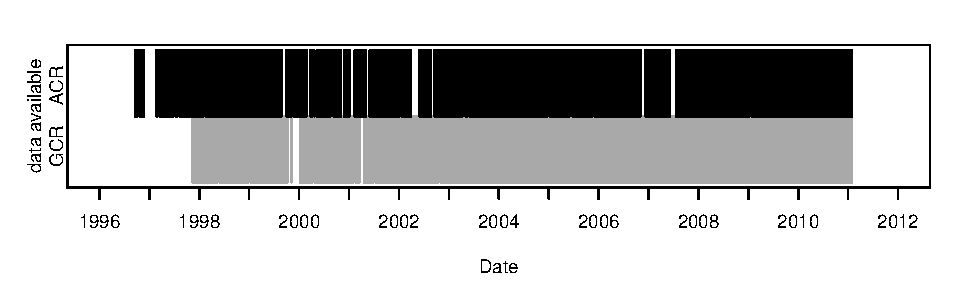
\includegraphics[width=6in]{figures/data_avail.pdf}
    \vspace{-2em}\\
    \caption{Available data}
    \label{fig:avail_data}
\end{singlespace}
\end{centering}
\end{figure}

As illustrated, data from both reports is generally available from November 1997
until January 2011, with a few relatively minor gaps. The period where the ACR
and GCR data overlap is the period used to analyze the effects of the CIDR
Report on AS behavior.

%	- plot total prefixes in the total table (Routeviews) and in the report (CIDR Report) to see that there aren't any discontinuities
% this is the "peer count" that I allude to

\subsection{GCR implementation quality}

In addition to data availability, the accuracy of the analysis that follows also
depends on the accuracy of our implementation of the CIDR Report aggregation
algorithm described in Chapter \ref{chap:method}. Recall that while the ACR is
used to determine when an AS appears on the CIDR Report (and thus potentially
commands attention of the community), the GCR is used to determine actual
post-appearance behavior because it provides consistently-generated measures
(like the number of aggregable prefixes advertised, \emph{netgain}) for ASes
both above and below the ACR top 30 threshold.

The first measure of accuracy is a comparison of the aggregable and total
prefixes determined for each AS on the ACR and GCR. A plot illustrating this
comparison is shown in Figure \ref{fig:comp_prefix_error}. The curves above the
horizontal zero ($y=0$) represent the sum of the differences in prefix counts
between the ACR and GCR for ASes where the GCR reports more prefixes than the
ACR. Similarly, the curves below the zero represent the sum of differences in
prefix counts between the ACR and GCR for ASes where the ACR reports more
prefixes than the GCR. The total deviation between the ACR and GCR is
given by the difference between the curves above and below zero.

\begin{figure}[h!]
\begin{centering}
\begin{singlespace}
    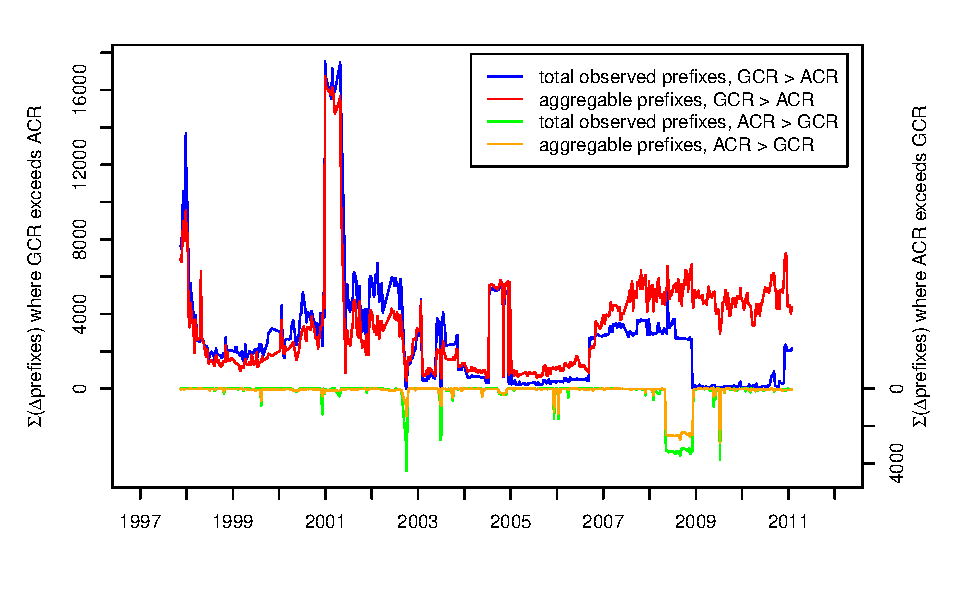
\includegraphics[width=6in]{figures/cidr_report_validity_prefix_error.pdf}
    \vspace{-2em}\\
    \caption{Differences in prefix counts between authoritative (ACR) and
        generated (GCR) CIDR Reports over time.}
    \label{fig:comp_prefix_error}
\end{singlespace}
\end{centering}
\end{figure}

As can be seen in Figure \ref{fig:comp_prefix_error}, throughout the period of
available data, the GCR generally claims larger quantities of aggregable and
total prefixes than the ACR. This is particularly pronounced and erratic when
compared against the pre-August 2002 CIDR Report (the point when the report's
methodology was changed when it was re-implemented by Geoff Huston). It is
difficult to determine the cause of this, but we suspect it is due to the
greater number of vantage points used in generating the GCR, leaving the GCR
more open to observing prefixes not visible from the ACR vantage point, or
observing AS\_PATHs that enable classification of prefixes as aggregable.

After August 2002, agreement between the ACR and GCR improves, though there are
still inconsistencies. Most of these inconsistencies appear attributable to
the GCR observing more prefixes than the ACR---this is the case when the
observed prefixes (blue line) and aggregable prefixes (red line) increase
simultaneously. Perhaps more concerning in terms of accuracy is the change in
behavior that began in late 2008 and continues to the latest, where the ACR and
GCR observe the same number of prefixes (blue line is approximately zero) but
the GCR classifies 4000-5000 more prefixes as aggregable.
\fbox{TODO: insert note from notebook from when I looked into this}

In spite of these inconsistencies, which are generally minor in terms of
ACR-GCR disparity for individual ASes, the GCR presents a view of potential
routing table aggregability that is sufficiently consistent with the ACR to
enable our use of the GCR as a data source for analyzing individual AS
aggregation behavior after appearing on the CIDR Report. Further, the
principles by which the GCR classifies prefixes as aggregable, as described in
the previous chapter, appear to be reasonable and sound from a technical
perspective. Finally, as will be discussed next, these minor differences in
prefix counts do not greatly affect the ranks of ASes on the GCR when compared
to the ACR.

While it is helpful to look at differences in prefix counts, as this is the
major purpose for which the GCR is used (rather than the ranking it generates),
we can also compare the rankings it generates against the rankings from the ACR
to compare the relative accuracy of the GCR. Ranks provided by the GCR are not
currently used in this analysis, so I only briefly raise this before continuing
on.

Figure \ref{fig:comp_rank_error} illustrates the minimum and maximum absolute
differences between the ranks of ASes appearing on the ACR and the ranks of
corresponding ASes on the GCR.

\begin{figure}[h!]
\begin{centering}
\begin{singlespace}
    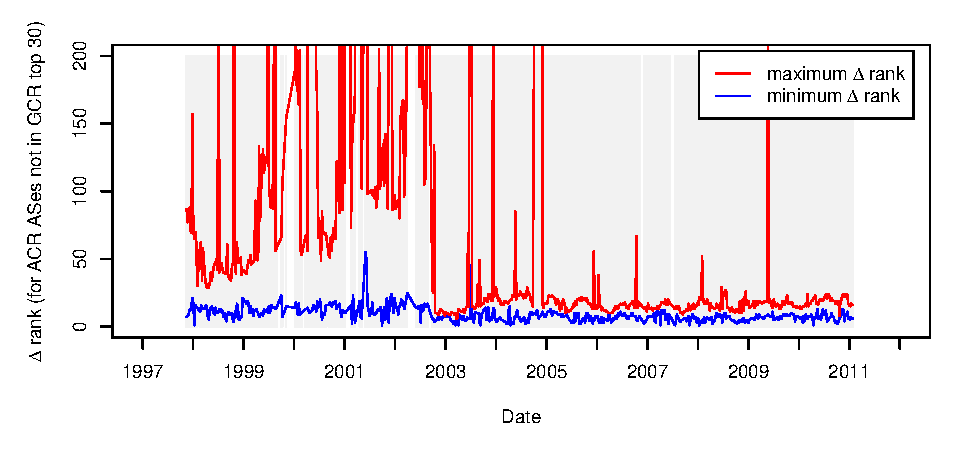
\includegraphics[width=6in]{figures/cidr_report_validity_rank_error.pdf}
    \vspace{-2em}\\
    \caption{Minimum and maximum differences in ASes ranked in the top 30 on
        the ACR but not in the top 30 on the GCR.}
    \label{fig:comp_rank_error}
\end{singlespace}
\end{centering}
\end{figure}

As can be seen, similar to the differences in prefix counts shown in the
previous figure, the rank differences are more significant and erratic from
1997 until August 2002, at which point they become more consistent. With some
exceptions, likely due to input data aberrations, the rankings generally differ
only a small amount, often near zero in the best case and no more than 20-30
in the worst case. Also, typically 20-25 of the ASes that appear on the ACR
also appear on the GCR (this is shown in a figure I may throw in the appendix).

% Figure \ref{fig:comp_top30_error} illustrates the total number of ASes ranked
% in the top 30 of the ACR that are not also in the top 30 of the GCR, as well as
% the rank of the first AS on the ACR not in the top 30 of the GCR.
%
% \begin{figure}[H]
% \begin{centering}
% \begin{singlespace}
%     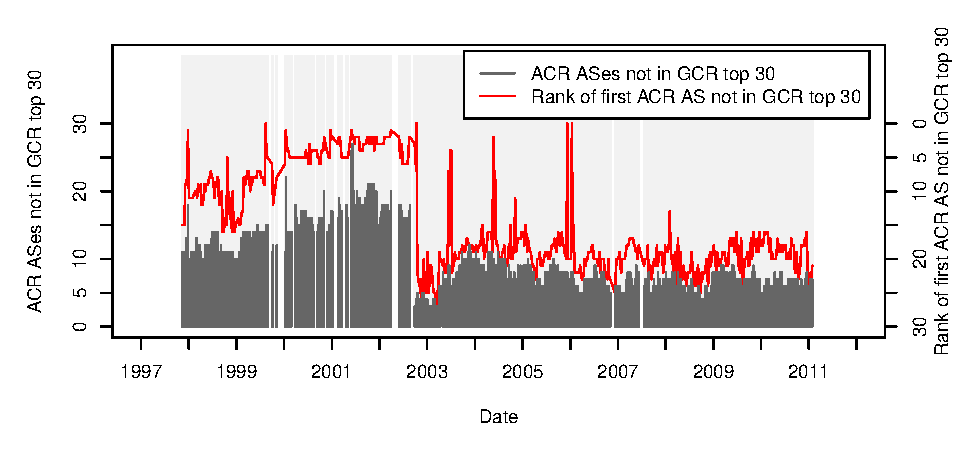
\includegraphics[width=6in]{figures/cidr_report_validity_top30_error.pdf}
%     \vspace{-2em}\\
%     \caption{The number and first rank of ASes in the treatment group (top 30)
%         of the ACR that are not in the treatment group of the GCR over time.}
%     \label{fig:comp_top30_error}
% \end{singlespace}
% \end{centering}
% \end{figure}

It was difficult to develop an implementation of the CIDR Report aggregation
algorithm (which is used to produce the GCR) that exactly matches the output of
the authoritative CIDR Report. Further, it is questionable whether an
implementation of the algorithm should strive to reproduce the output of a
``black box'' (even if it is the black box that is used to inform and influence
the operator community) instead of being based on first principles and a
conceptual understanding of the purpose of the CIDR Report. For these reasons,
along with the fact that the GCR is reasonably in agreement with the ACR, we
believe it is reasonable to use this data in our analysis.

\section{Characteristics of the CIDR Report}
In analyzing the CIDR Report, much time was spent looking at characteristics of
the report and networks that appear on it. While this was not directly related
to answering the question of whether appearing on the CIDR Report changes route
aggregation behavior, it is useful in providing context about the CIDR Report,
and also possibly offering insights about the causes of the behavior changes
that are observed in answering the question of this thesis. The characteristics
discussed in this section are organized into two categories: relative measures
of network behavior on the CIDR Report (typically related to ranks and ranking)
and absolute measures of network behavior (typically related to prefixes
advertised).

\subsection{AS Appearances and rank-based observations}
The first approach taken to gain an understanding of the behavior of the CIDR
Report was to visualize it in a two-dimensional space, with time in one
dimension and CIDR Report rank in the other dimension. An excerpt of this
visualization is shown in Figure \ref{fig:viz_sample}.

\begin{figure}[h!]
\begin{centering}
\begin{singlespace}
    \includegraphics[width=4in]{figures/viz_sample.jpg}
    \caption{Visualization sample.}
    \label{fig:viz_sample}
\end{singlespace}
\end{centering}
\end{figure}

This visualization was not especially practical, as it was physically large and
the level of detail and limited range of colors available made it difficult to
visually identify and distinguish the behaviors of individual ASes. However,
this visualization provided some clues about interesting characteristics to
investigate. By visual inspection, it appeared as though the CIDR Report was
volatile at lower ranks but relatively static near the top (most aggregation
potential). It also appeared that the report was more volatile in the past but
become more static overall more recently. These and other aspects were then
investigated using analytic techniques, which are described and presented next.

A number of interesting characteristics about the CIDR Report are of a
demographic nature, such as how many ASes appear on the CIDR report, or for how
long do ASes remain on the report? This first question, about how many ASes
ever appear on the CIDR Report, is illuminated by Figure \ref{fig:as_counts}.

\begin{figure}[h!]
\begin{centering}
\begin{singlespace}
    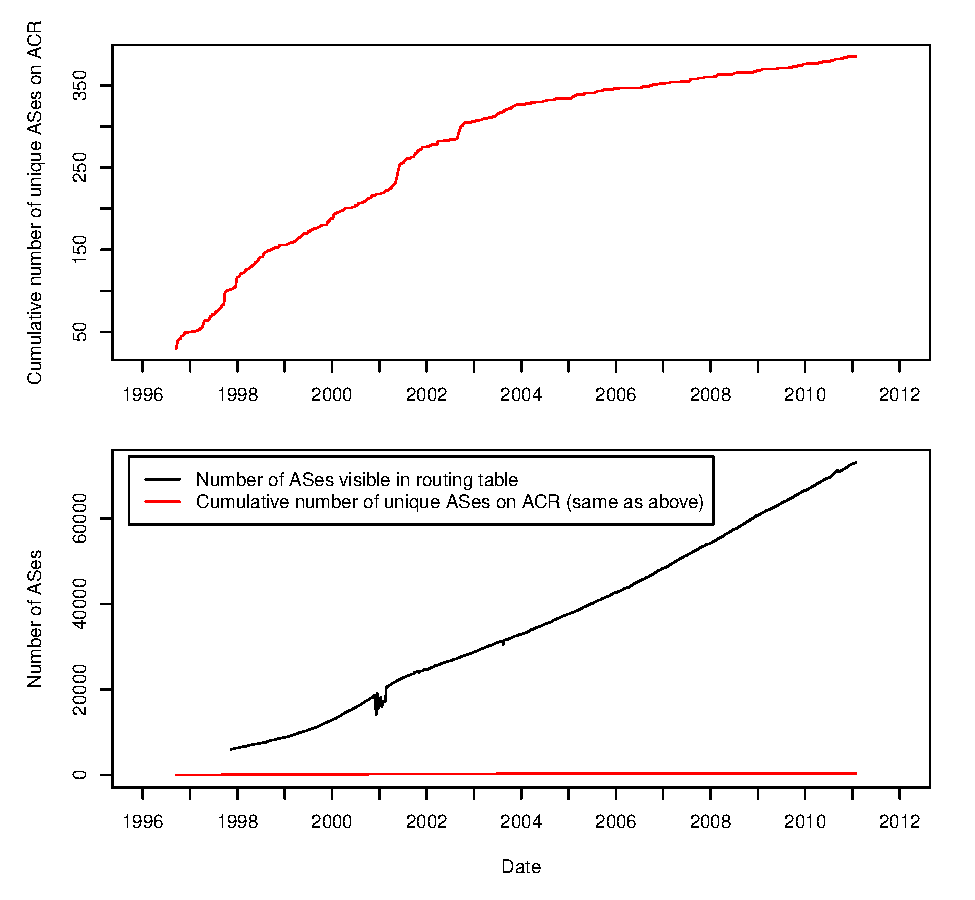
\includegraphics[width=6in]{figures/cumulative_asn_counts.pdf}
    \vspace{-2em}\\
    \caption{A cumulative count of the unique ASes that have appeared on the
        CIDR Report and compared to the cumulative count of unique ASes visible
        in the routing table up to the same point.}
    \label{fig:as_counts}
    %TODO: in future, think about plotting unique ASes ever appearing within
    %certain rank slots.
\end{singlespace}
\end{centering}
\end{figure}

In this figure, the top plot shows the cumulative number of ASes that appear on
the CIDR Report, starting with 30 ASes on the first report in 1996 and
concluding with 386 unique ASes in 2011. The growth of new ASes appearing on
the report appears to be greater in the late 1990s and early 2000s than in the
mid-late 2000s. More remarkable is how relatively few ASes from the total set
of ASes that ever appear in the Internet routing table appear on the CIDR
Report. This relationship is shown in the bottom plot of Figure
\ref{fig:as_counts}. In this figure, the red curve near the bottom of the graph
area is the same red curve that was plotted in the upper figure, and the black
curve that rises steadily is the total number of ASes visible in the routing
table. This illustrates that less than 1\% of all ASes have ever appeared on
the CIDR Report.

While the former plot illustrated the total number of ASes that appear on the
report, it does not provide any information about how long an AS appears on the
report for. This information is provided in the next figure. Figure
\ref{fig:cdf_weeks}, which presents a cumulative distribution function of the
total number of weeks each AS appears on the CIDR Report. Noting the log scale
on the x-axis, we can see that 15\% of all ASes that appear on the CIDR Report
are on the report for only a single week, half of all ASes are on the report
for approximately 10 weeks or less, and that there is a general exponential
relationship between increasing fractions of the population and time spent
on the report (i.e. for each 10\% increase in population considered, the
maximum duration spent on the report doubles).

\begin{figure}[h!]
\begin{centering}
\begin{singlespace}
    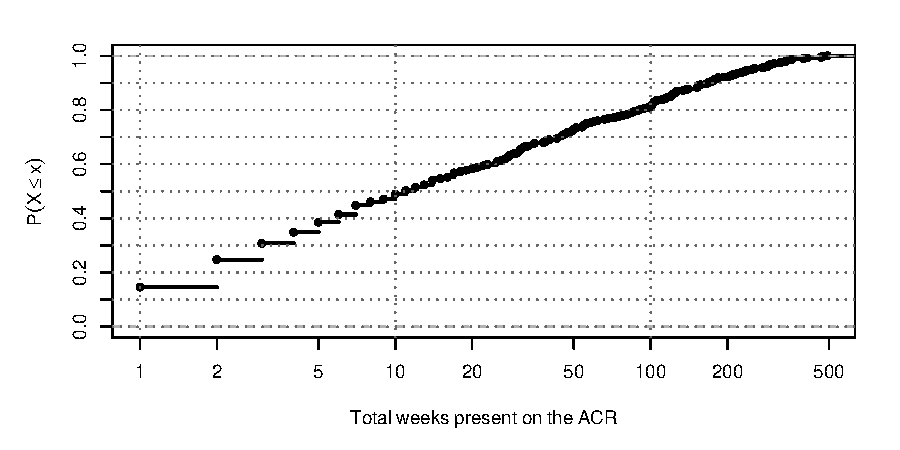
\includegraphics[width=6in]{figures/acr_cdf_weeks.pdf}
    \vspace{-2em}\\
    \caption{A cumulative distribution function of the total number of weeks
        that each AS is visible on the CIDR Report.}
    \label{fig:cdf_weeks}
\end{singlespace}
\end{centering}
\end{figure}

%TODO: tempting to take the following graf and figure out.
% A similar plot with a different metric is shown in Figure
% \ref{fig:cdf_rankweeks}. In this figure, instead of presenting the number of
% weeks each AS spends on the report, the number of rank-weeks accrued by each AS
% are displayed instead. A rank week is simply the sum of the ranks an AS
% occupies for each week it appears on the CIDR Report. So an AS could accumulate
% a rank-week measure of 100 by spending 100 weeks at the very bottom of the
% report (rank of 1, 30th position) or 10 weeks at a rank of 10 (20th position).
%
% \begin{figure}[h!]
% \begin{centering}
% \begin{singlespace}
%     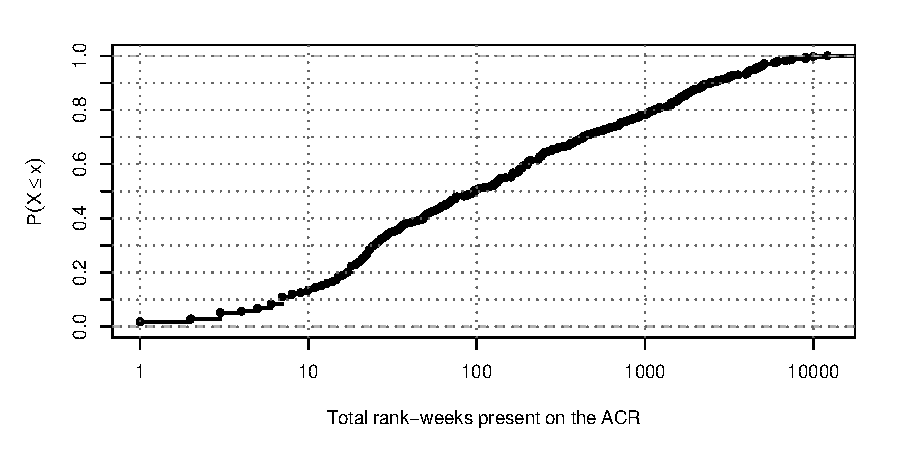
\includegraphics[width=6in]{figures/acr_cdf_rankweeks.pdf}
%     \vspace{-2em}\\
%     \caption{A cumulative distribution function of the total number of
%         rank-weeks that each AS is visible on the CIDR Report.}
%     \label{fig:cdf_rankweeks}
% \end{singlespace}
% \end{centering}
% \end{figure}

This is the first indication that not all the ASes that appear on the CIDR
report behave in similar ways, but instead that many ASes appear only briefly
in comparison to some ASes that occupy a considerable part of the CIDR Report.

% \begin{figure}[H]
% \begin{centering}
% \begin{singlespace}
%     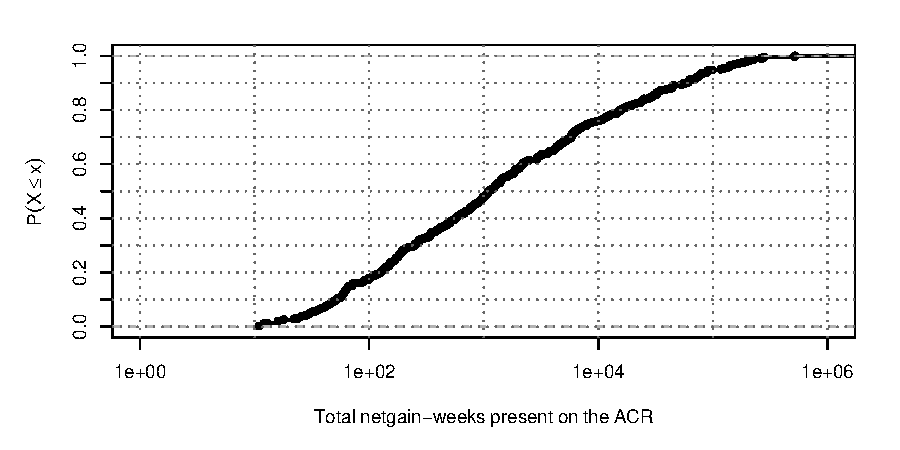
\includegraphics[width=6in]{figures/acr_cdf_ngweeks.pdf}
%     \vspace{-2em}\\
%     \caption{A cumulative distribution function of the total number of netgain-weeks that each AS is visible on the CIDR Report.}
% \end{singlespace}
% \end{centering}
% \end{figure}

Returning to the observation from earlier that the top ranks of the CIDR Report
are static relative to the volatile lower ranks, we investigated this further
by plotting cumulative distribution functions of the number of weeks that a
particular AS occupies a given rank on the CIDR Report. These plots, for ranks
1 (most potential for aggregation) to 30, are shown in groups in Figure
\ref{fig:rank_cdfs}

\begin{figure}[h!]
\begin{centering}
\begin{singlespace}
    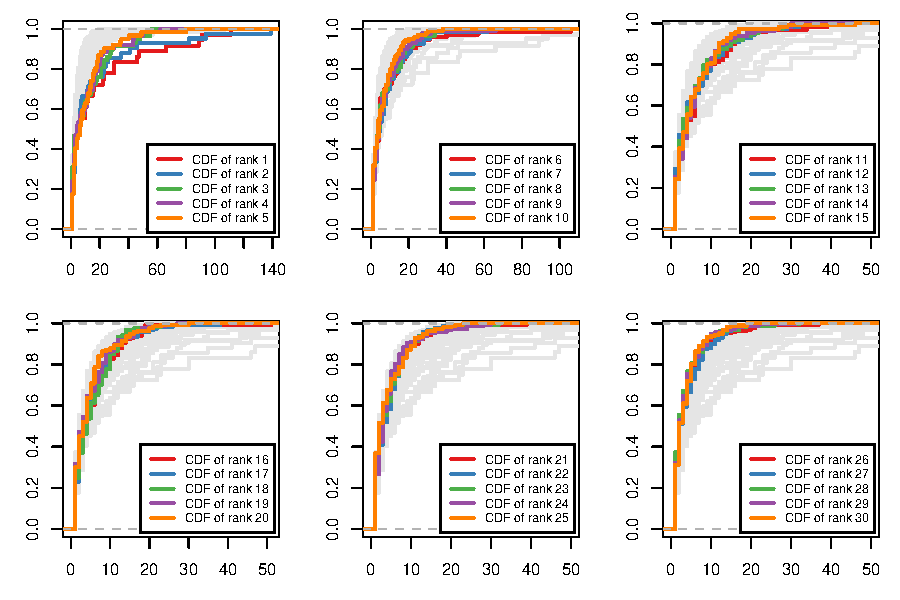
\includegraphics[width=6in]{figures/cr_rank_cdfs.pdf}
    \vspace{-2em}\\
    \caption{CDFs of the number of weeks that a given rank was occupied by a
    single AS. The x-axis is the number of weeks, and the y-axis is the
    fraction of the population. The light gray lines indicate CDFs of other
    ranks, in order to place the highlighted ranks in context.}
    \label{fig:rank_cdfs}
\end{singlespace}
\end{centering}
\end{figure}

As illustrated clearly by this figure, lower ranks on the CIDR Report are more
volatile than top ranks. The top five positions, ranks 1-5, are particularly
ossified, with the top 10\% of ASes that ever appear occupying individual ranks
for no less than 20-60 weeks. In contrast, the lower ranks, and particularly
the bottom half (ranks lower than 15) are much more volatile, with around
90\% of the AS population occupying a given rank for 10 weeks or less, and
essentially all of the population not occupying ranks for more than 20
weeks. This is consistent with the claimed observation of operators that
the CIDR Report does not appear to change much---especially the top ranks
that are first visible in the email. What appears to be the apparent reason
for this ossification will be discussed in the next section.

\subsection{Prefix-based observations}

%TODO: include a figure of the proportion of the routing table that is
%aggregable/deaggregated over time? Plot deagg_factor or frac_aggr?

While the previous section made some interesting observations about ASes'
appearance and movement behavior through the CIDR Report, it was focused on the
relative measures of AS rank (and relatedly, appearance within the top 30) on
the CIDR Report. It is also helpful to gain a perspective about characteristics
of the CIDR report considering the prefixes that each AS is advertising, as
prefix counts (and routing table slots) are ultimately the metric that is
important in considering behavior change in the context of the routing table.

Figure \ref{fig:netcompare}\footnote{All data in this plot is from the GCR, but
classification of an AS and its netgain/netsnow figures are based on the ASes
present on the ACR as emailed. Data from the GCR is used to allow for consistent
comparison between the entire routing table and the top 30 (ACR) ASes.}
illustrates what fraction of the the total prefixes and aggregable prefixes
visible in the Internet routing table are advertised by ASes appearing on the
CIDR Report.

\begin{figure}[h!]
\begin{centering}
\begin{singlespace}
    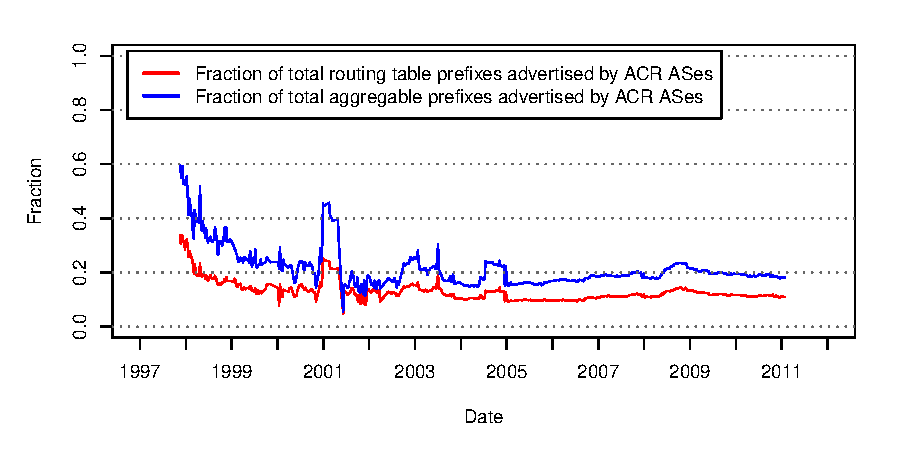
\includegraphics[width=6in]{figures/acr_gcr_netcompare2.pdf}
    \vspace{-2em}\\
    \caption{Plots of the fractions of total prefixes and total aggregable
    prefixes in the routing table that are advertised by ASes appearing on the
    CIDR Report.}
    \label{fig:netcompare}
\end{singlespace}
\end{centering}
\end{figure}

This figure suggests that in the past, the CIDR Report did indeed focus quite
effectively on the ``worst offenders'' in terms of networks advertising
aggregable routes---at the beginning of the period of available data, it
captured nearly 60\% of the total aggregable routes in the top 30 list. This
has dropped off and, interestingly, remained approximately proportional to the
growth of the routing table since 2003 or 2004, suggesting that growth of
deaggregation in the ASes at the top of the CIDR Report is proportional to the
growth of deaggregation across the Internet routing table. However, as the next
figure will show, this proportionality has been maintained in the face of
growth of the number of participants in the Internet routing table, such that
the ASes that appear at the top of the report have become disproportionally
deaggregated.

Another way of considering how the prefix advertisement behaviors of networks
on the CIDR Report relates to other networks in the routing table is to look at
the distribution of deaggregation (advertisement of aggregable prefixes) in the
routing table. Cumulative distribution functions of aggregable prefixes
(netgain) visible in the routing table (from the GCR) over time is shown in
Figure \ref{fig:netgain_cdf}.

% TODO in future, look into whether the distribution of deaggregators is a
% power-law relationship
\begin{figure}[h!]
\begin{centering}
\begin{singlespace}
    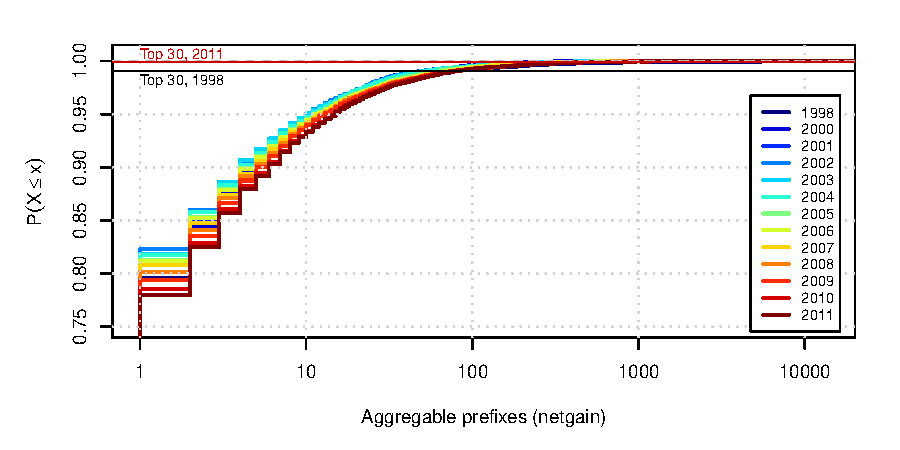
\includegraphics[width=6in]{figures/netgain_cdf_gcr.pdf}
    \vspace{-2em}\\
    \caption{CDFs of netgain of all ASes in the routing table in the first week
    of the year from 1998-2011. Threshold lines indicating the cutoff point for
    appearing on the CIDR Report in 1998 and 2011 are indicated. Note that the
    graph is rescaled; approximately 70\% of ASes in the routing table do not
    advertise any aggregable prefixes.}
    \label{fig:netgain_cdf}
\end{singlespace}
\end{centering}
\end{figure}

From these distributions we can see that while advertisement of aggregable
prefixes has increased slightly across the routing table over time, as given by
the downward move in the CDF curves over time, the distribution of aggregable
prefixes announced by ASes has remained roughly similar, with an increasingly
long long-tail of outliers in the top fraction of a percentile of the
population of ASes. This figure is potentially misleading, as while the
distribution of aggregable prefix announcement has not changed, the total
number of ASes visible in the routing table has grown over time, from 3172 ASes
in the first week of 1998 to 36383 ASes in the first week of 2011. Thus, there
are approximately ten times the number of ASes announcing the same number of
aggregable prefixes now than in 1998.

What is also noteworthy in this figure is the indication of
the threshold points for appearing on the CIDR Report in 1998 and 2011. The
fraction of the population above this line is the ``top 30'' group that would
appear on the CIDR Report. This line appears to have moved from approximately
1\% of the population to some small fraction of a percent. This conclusion
follows from the fact that the number of ASes in the routing table has grown
over time and yet the length of the CIDR report has remained the same. However,
as this figure, as well as Figure \ref{fig:netcompare} illustrate, this also
means that the CIDR Report has changed to highlight mostly outlier behavior,
leaving the individually less significant but collectively more significant
deaggregation below the threshold unaddressed.

% \begin{figure}[H]
% \begin{centering}
% \begin{singlespace}
%     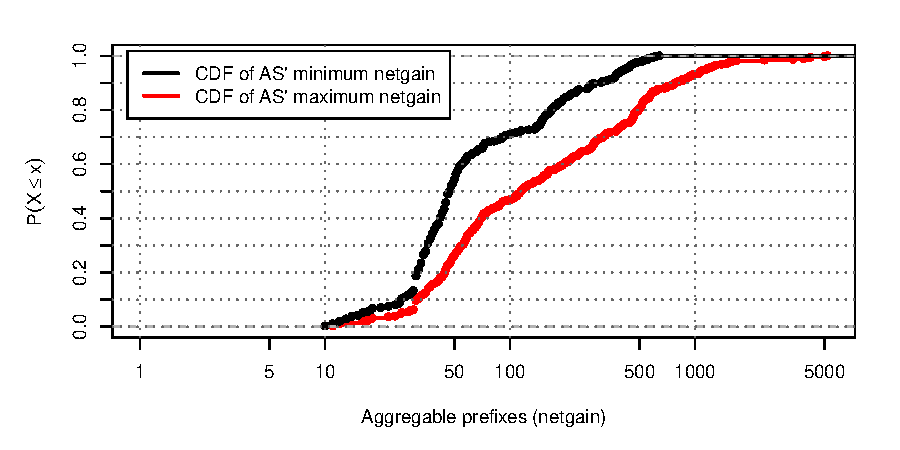
\includegraphics[width=6in]{figures/acr_netgain_cdfs.pdf}
%     \vspace{-2em}\\
%     \caption{CDFs of the minimum and maximum netgain observed for each AS during its time on the CIDR Report.}
% \end{singlespace}
% \end{centering}
% \end{figure}

The question of where the threshold to appear on the CIDR Report is---how much
deaggregation it takes for an AS to appear on the report---is addressed in
Figure \ref{fig:thresholds}. This figure displays the minimum netgain
thresholds to appear on the CIDR Report (rank 30) as well as the median (rank
15) and various other top ranks.

\begin{figure}[h!]
\begin{centering}
\begin{singlespace}
    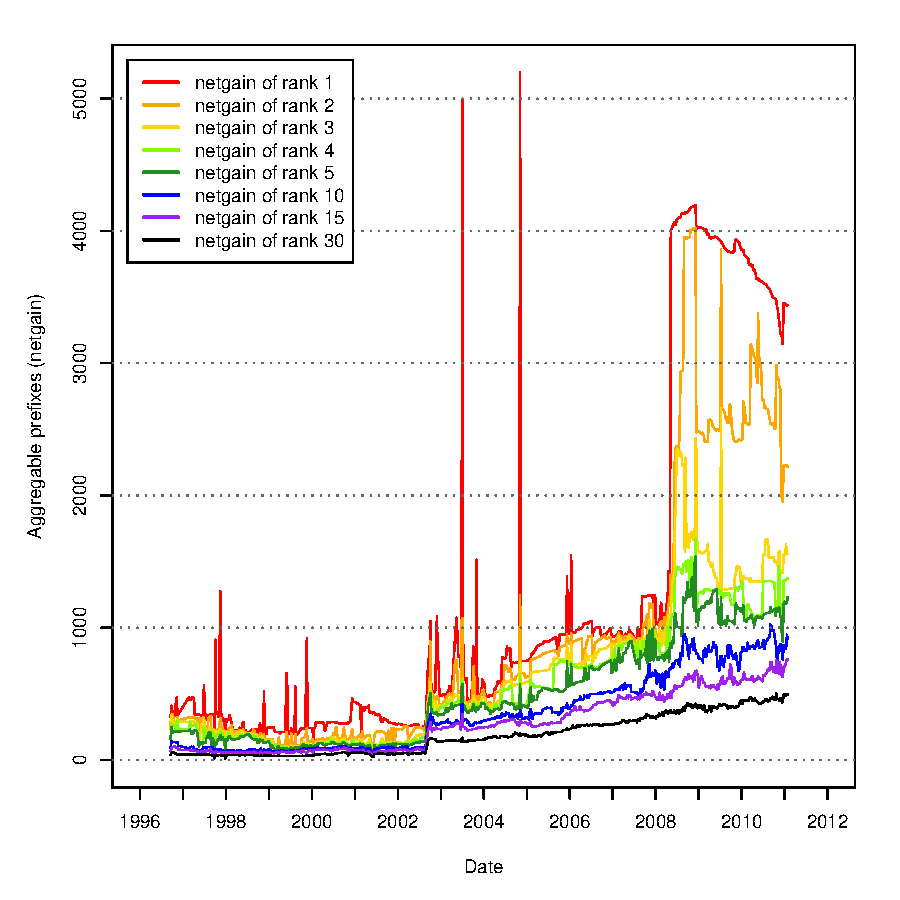
\includegraphics[width=6in]{figures/acr_netgain_time.pdf}
    \vspace{-2em}\\
    \caption{The netgain thresholds required to achieve indicated ranks on the
    ACR over time.}
    \label{fig:thresholds}
    \end{singlespace}
\end{centering}
\end{figure}

This figure of the CIDR Report rank thresholds shows an increasing spread in
prefix thresholds for the various ranks over time, particularly in the top 5,
as well as between the top 5 and the median, compared to between the median and
the minimum threshold (rank 30). The increasing spread between ranks can also
be viewed in a slightly different way, with a focus on temporal progression, in
the following figure. Figure \ref{fig:netgain_cdf_acr} presents cumulative
distribution functions of the number of aggregable prefixes (netgain)
advertised by each AS on the ACR in the first week of the year indicated.

\begin{figure}[h!]
\begin{centering}
\begin{singlespace}
    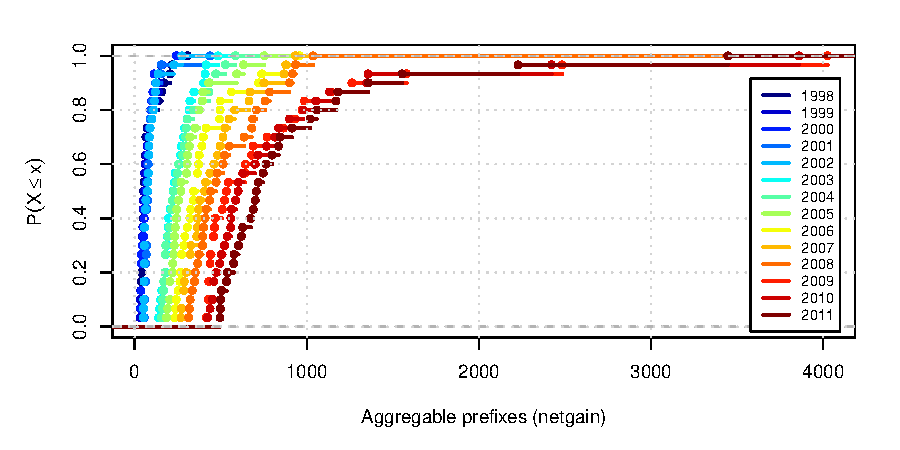
\includegraphics[width=6in]{figures/netgain_cdf_acr.pdf}
    \vspace{-2em}\\
    \caption{Plots of CDFs of the netgain of the ASes visible on the ACR in the
    first week of each year 1998-2011. Notice that the top of the population
    spreads more in later years.}
    \label{fig:netgain_cdf_acr}
\end{singlespace}
\end{centering}
\end{figure}

Here again we see the growing spread between ranks and the changing shape of
the distribution as ASes at the top of the report differ from the bottom more
in later years than in previous years. Both this and the previous plot suggest
that the ossification in the top ranks of the CIDR report observed earlier are
due to the growing spread in netgain, making it more difficult to ``unseat''
high-ranked ASes because they are so far from the next nearest AS (in terms of
number of prefixes). This is not necessary a problem, and also our measure of
volatility may be imperfect (i.e. an AS could oscillate between two ranks,
appearing volatile even though its behavior does not chance perceptibly), but
this does provide some explanation for the static behavior noted before.

% Finally, just because it is interesting, I include a plot of the minimum
% threshold, in terms of aggregable prefixes, that are necessary to appear on the
% CIDR Report over time.
%
% %TODO should I include this???
% \begin{figure}[H]
% \begin{centering}
% \begin{singlespace}
%     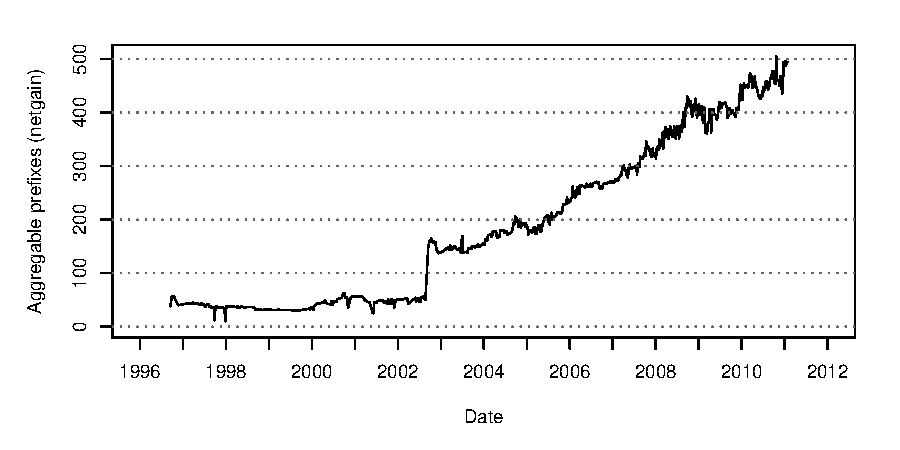
\includegraphics[width=6in]{figures/acr_netgain_time_min.pdf}
%     \vspace{-2em}\\
%     \caption{A plot of the minimum netgain required to appear on the CIDR
%     Report over time.}
%     \end{singlespace}
% \end{centering}
% \end{figure}

%TODO should I include this???
% \begin{figure}[h!]
% \begin{centering}
% \begin{singlespace}
%     \includegraphics[width=6in]{figures/netgain_frac_aggr_cdf_gcr.pdf}
%     \vspace{-2em}\\
%     \caption{Plots of CDFs of the fraction of prefixes announced by each AS
%     that are aggregable, over time.}
%     \label{fig:netgain_cdf_acr}
% \end{singlespace}
% \end{centering}
% \end{figure}

\subsection{Conclusions}

Both these observations of characteristics of the CIDR Report related to the
number of prefixes advertised by each AS, as well as the previous observations
about the rank of each AS and appearance of ASes on the CIDR Report, suggest
that while the advertisement of redundant, aggregable prefixes in the routing
table is reasonably commonplace, the ASes that appear on the CIDR Report are
outliers in that they announce significantly more aggregable prefixes than most
of the rest of the population of ASes participating in the interdomain routing
system. In its earlier days the CIDR Report captured a larger fraction of the
ASes responsible for aggregable prefixes than it does now, because of
growth in the number of ASes announcing aggregable routes, and the top of the
report seems to have become relatively static because of the extreme
deaggregation of ASes at the top of the report relative to the majority of the
AS population.

\section{Analysis of AS behavior after appearing on the CIDR Report}

This section presents and discusses the results of the primary question of this
thesis, \emph{do autonomous systems change their behavior, as measured by the
number of aggregable routes they advertise into the routing table (netgain),
after appearing on the CIDR Report?} As described in section
\ref{sec:method_agg_report_analysis}, data from the CIDR Report is processed to
determine when ASes first appear on the report, and samples are then take from
30 to 730 days after this initial appearance (detailed in Figure
\ref{fig:sample_ex}) and compared to the value at the time of first appearance.
Decreases in netgain would suggest that the CIDR Report does influence network
operator route aggregation behavior in the expected or intended way, while no
change or increased netgain would suggest that the CIDR Report has no effect.
The group of ASes appearing on the CIDR Report, and thus theoretically subject
to social forces to improve aggregation behavior, will hereafter be referred to
as the treatment group.

In an attempt to control for normal variation in AS behavior that does not
result from appearing on the CIDR Report, a ``control group'' was established
from ASes never appearing on the CIDR Report, as described in much more detail
in section \ref{sec:method_agg_report_analysis}, to determine the behavior of
ASes that are not treated by the CIDR Report. As this is a quasi-experiment
rather than a randomized, controlled experiment, this group will hereafter be
referred to as the ``untreated group'' instead.

A number of quantities are measured and presented in the following section, in
an effort to discern the behavior of ASes appearing on the CIDR Report. They
are as follows (in all cases, $t$ is symbolic of the time of first appearance,
and $k$ is one of the measurement time periods from 30-730 days):
\begin{itemize}
\item{Change in netgain: $\Delta\textrm{netgain}_{t+k} = \textrm{netgain}_{t+k}
    - \textrm{netgain}_{t+0}$}
\item{Relative change in netgain: $\frac{\Delta\textrm{netgain}_{t+k}}
    {\textrm{netgain}_{t+0}}$}
\item{Change in netsnow: $\Delta\textrm{netsnow}_{t+k} = \textrm{netgain}_{t+k}
    - \textrm{netsnow}_{t+0}$}
\item{Relative change in netsnow: $\frac{\Delta\textrm{netsnow}_{t+k}}
    {\textrm{netsnow}_{t+0}}$}
\item{Fraction of prefixes that are aggregable (``fraction aggregable''):
    $\frac{\textrm{netgain}_{t+k}} {\textrm{netsnow}_{t+k}}$}
% \item{Deaggregation factor: $\frac{\textrm{netsnow}_{t+k}}
%     {\textrm{netsnow}_{t+k} - \textrm{netgain}_{t+k}}$}
\end{itemize}

Note that the final quantity above, while a useful measure of deaggregation,
is not measured relative to the original appearance point, and so must be
viewed together with the fraction aggregable measure at the original point of
appearance ($t+0$) in order to observe change in behavior.

With this initial explanation, we are ready to present the results of our
analysis, beginning with netsnow and netgain, and followed with fraction
aggregable, which demonstrates the greatest observed behavior change. Unless
otherwise noted in captions of the figures or the associated text, all of the
following figures utilize all appearances on the CIDR Report from 1997-2011.
Figures of these quantities utilizing appearances from only a portion of the
date range, to discern changes in behavior over time, are included in Appendix
\ref{chap:additional_figs}.

\subsection{Change in netgain in response to CIDR Report appearance}

\begin{figure}[H]
\begin{centering}
\begin{singlespace}
    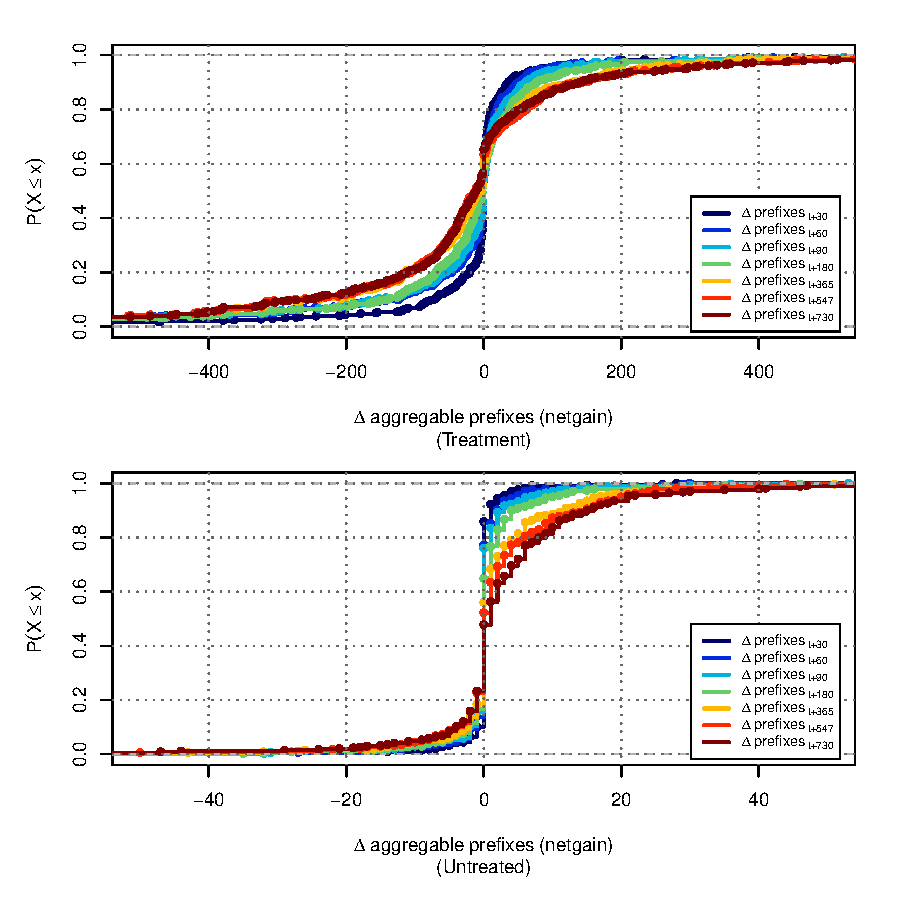
\includegraphics[width=6in]{figures/behavior-netgain-1997_2011-corr.pdf}
    \vspace{-2em}\\
    \caption{Cumulative distribution function of change in number of aggregable
    prefixes (netgain) advertised by treated and untreated (control) ASes, for
    the period 1997-2011.}
\end{singlespace}
\end{centering}
\end{figure}

\begin{figure}[H]
\begin{centering}
\begin{singlespace}
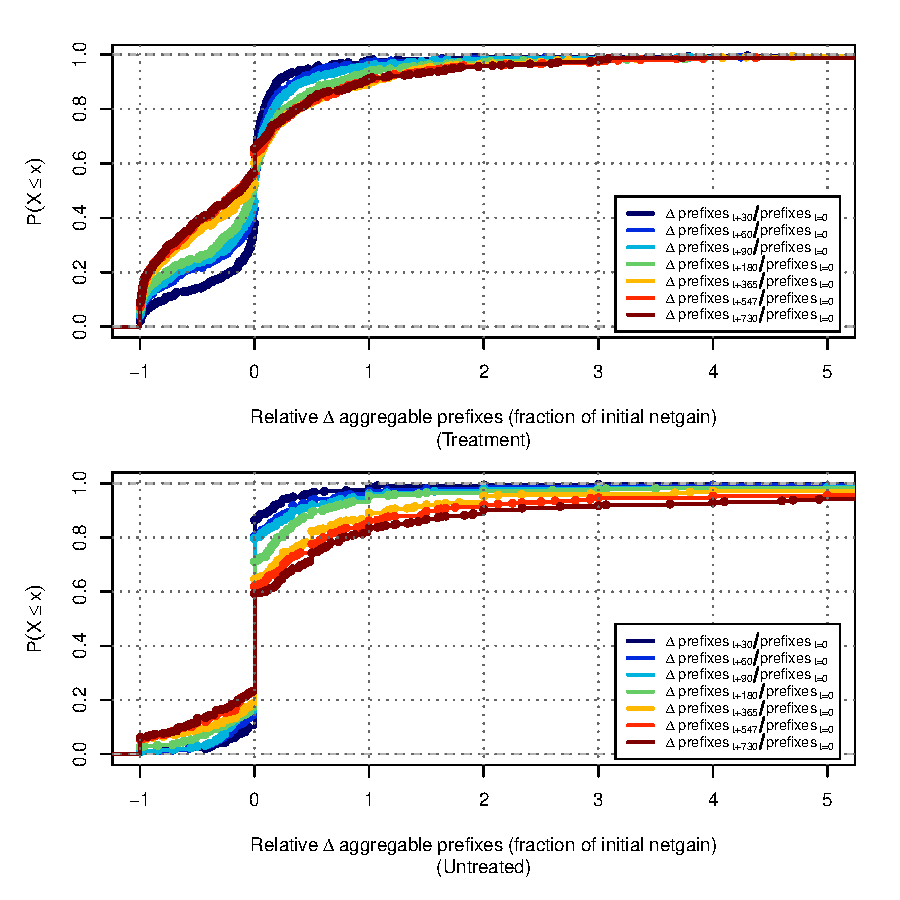
\includegraphics[width=6in]{figures/behavior-rel_netgain-1997_2011-corr.pdf}
    \vspace{-2em}\\
    \caption{Cumulative distribution function of relative change in number of
    aggregable prefixes (netgain) advertised by treated and untreated (control)
    ASes, for the period 1997-2011.}
\end{singlespace}
\end{centering}
\end{figure}

\subsection{Change in netsnow in response to CIDR Report appearance}

\begin{figure}[H]
\begin{centering}
\begin{singlespace}
    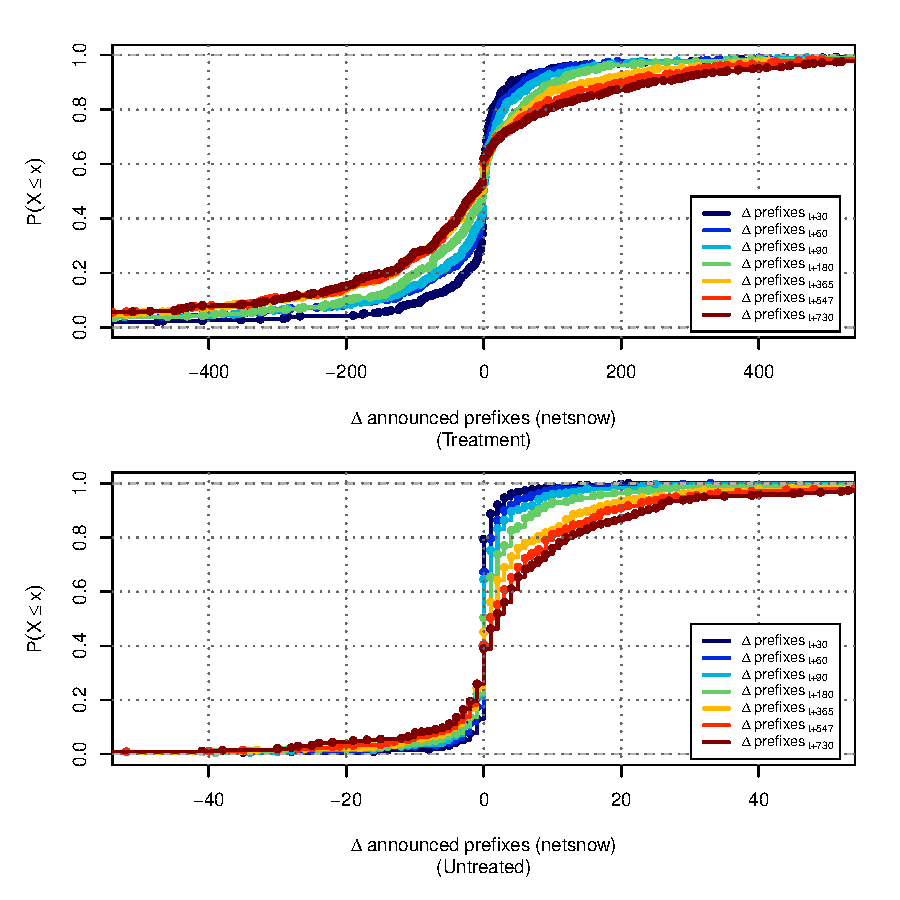
\includegraphics[width=6in]{figures/behavior-netsnow-1997_2011-corr.pdf}
    \vspace{-2em}\\
    \caption{Cumulative distribution function of change in total number of
    prefixes (netsnow) advertised by treated and untreated (control) ASes, for
    the period 1997-2011.}
\end{singlespace}
\end{centering}
\end{figure}

\begin{figure}[H]
\begin{centering}
\begin{singlespace}
    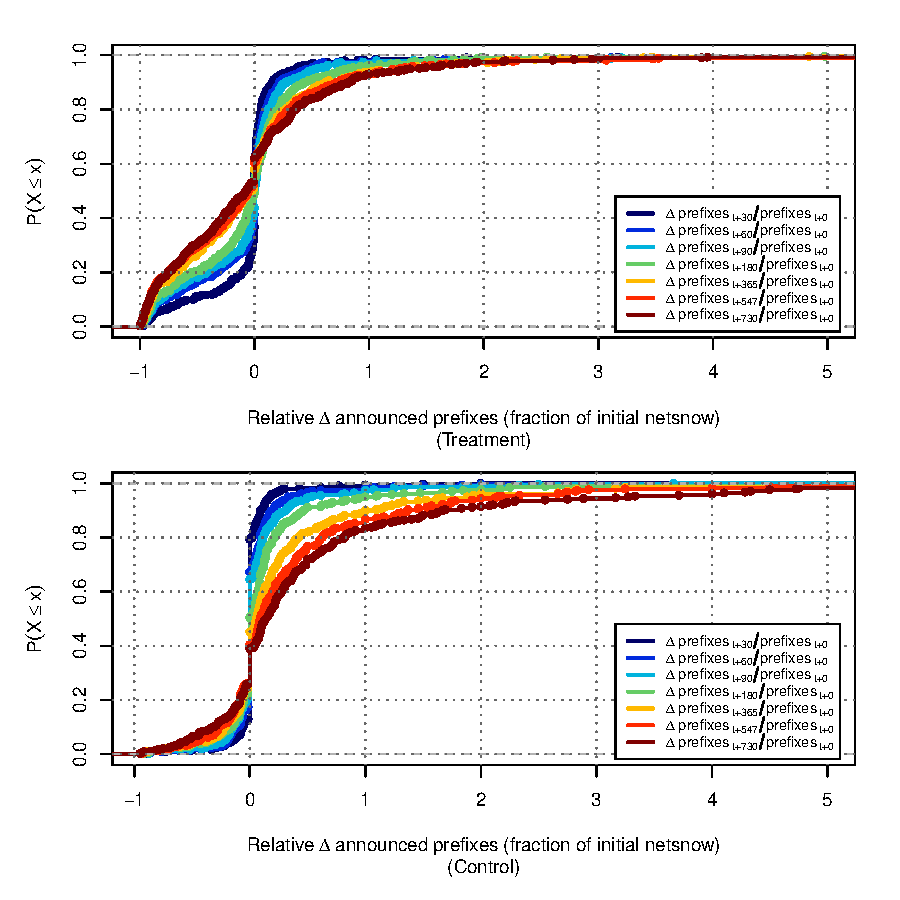
\includegraphics[width=6in]{figures/behavior-rel_netsnow-1997_2011-corr.pdf}
    \vspace{-2em}\\
    \caption{Cumulative distribution function of relative change in total
    number of prefixes (netsnow) advertised by treated and untreated (control)
    ASes, for the period 1997-2011.}
\end{singlespace}
\end{centering}
\end{figure}

\subsection{Change in fraction aggregable in response to CIDR Report appearance}

\begin{figure}[H]
\begin{centering}
\begin{singlespace}
    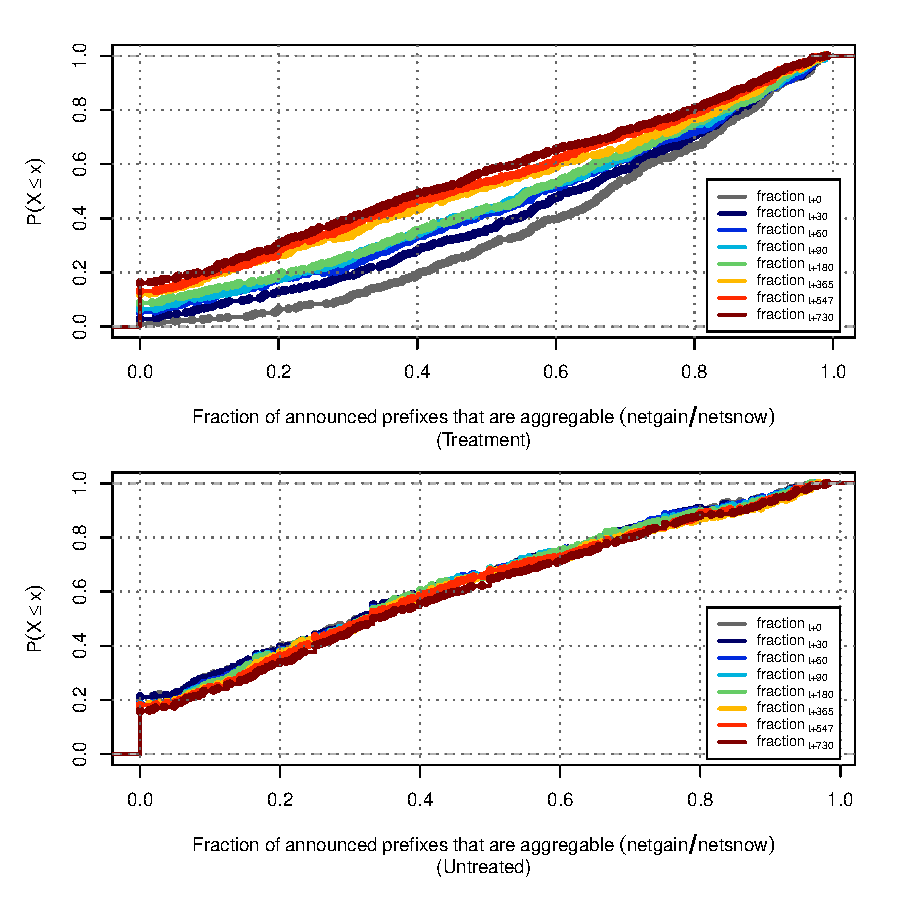
\includegraphics[width=6in]{figures/behavior-frac_deagg-1997_2011-corr.pdf}
    \vspace{-2em}\\
    \caption{Cumulative distribution function of change in the fraction of
    prefixes advertised by treated and untreated (control) ASes that can be
    aggregated without affecting routing policy, for the period 1997-2011.}
\end{singlespace}
\end{centering}
\end{figure}

\begin{figure}[H]
\begin{centering}
\begin{singlespace}
    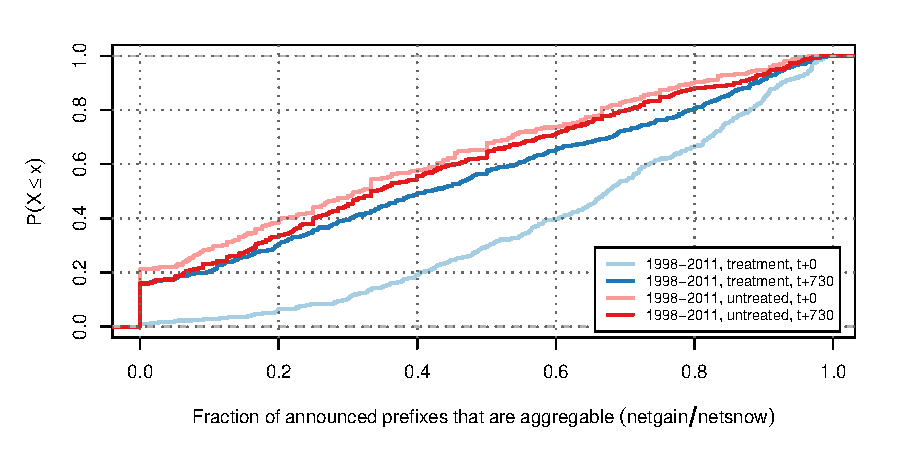
\includegraphics[width=6in]
        {figures/behavior-frac_deagg-1997_2011-special_tc.pdf}
    \vspace{-2em}\\
    \caption{Simplification of previous figure, showing the first (t+0) and
    last (t+730) CDF of the fraction aggregable for both the treatment and
    untreated groups.}
\end{singlespace}
\end{centering}
\end{figure}





\begin{figure}[H]
\begin{centering}
\begin{singlespace}
    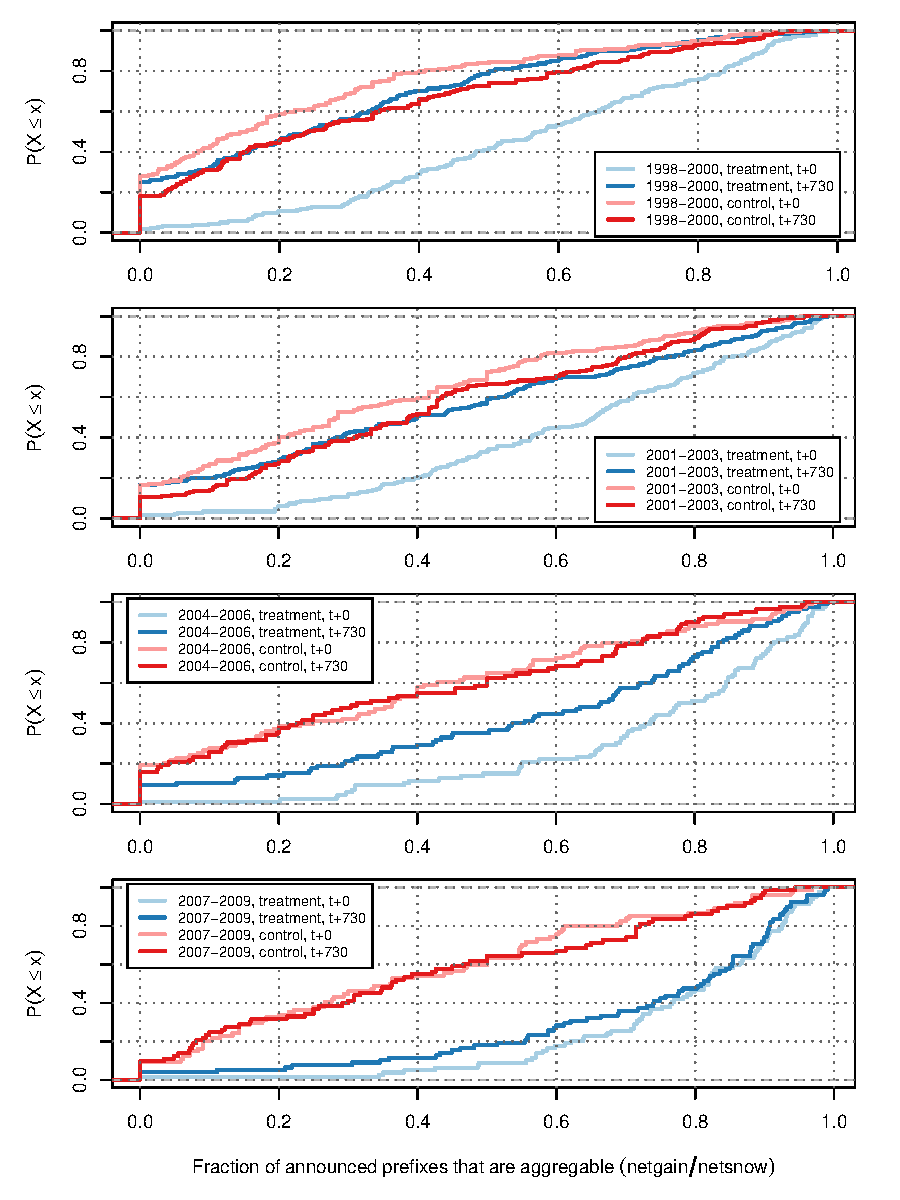
\includegraphics[width=6in]
        {figures/behavior-frac_deagg-vseries-special_tc.pdf}
    \vspace{-2em}\\
    \caption{}
\end{singlespace}
\end{centering}
\end{figure}





\begin{figure}[H]
\begin{centering}
\begin{singlespace}
    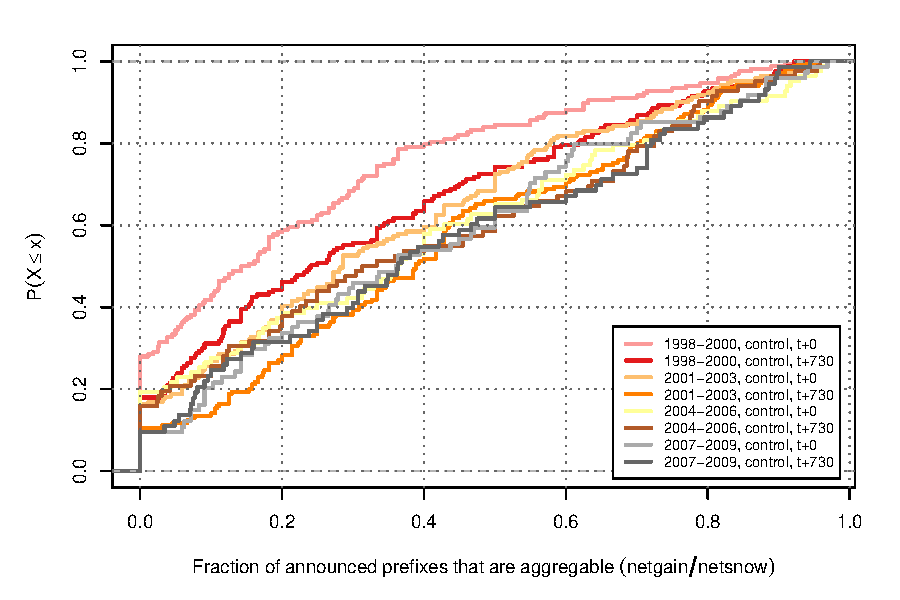
\includegraphics[width=6in]{figures/behavior-frac_deagg-all-special_c.pdf}
    \vspace{-2em}\\
    \caption{}
\end{singlespace}
\end{centering}
\end{figure}

\begin{figure}[H]
\begin{centering}
\begin{singlespace}
    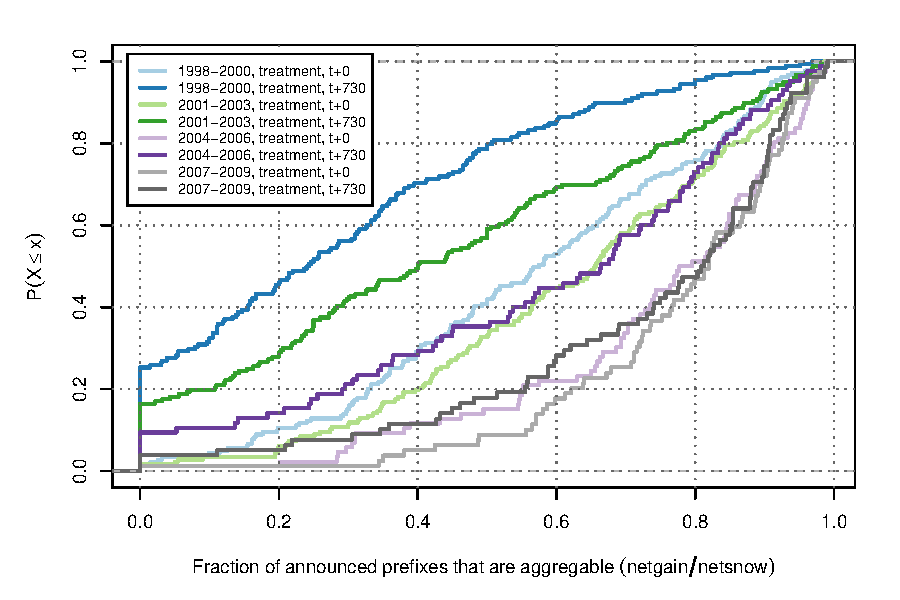
\includegraphics[width=6in]{figures/behavior-frac_deagg-all-special_t.pdf}
    \vspace{-2em}\\
    \caption{}
\end{singlespace}
\end{centering}
\end{figure}


\subsection{\fbox{TODO: Notes on validity}}
It is still difficult to tell whether the CIDR Report is having an effect -- how
do we know we are not measuring something else coincident with the CIDR Report?
This is difficult to address... Look at large-netsnow with low-netgain
population??? Future work.

It was an oversight that I did not measure behavior of ASes before their
appearance on the CIDR Report. However, because appearance is determined based
on netgain behavior means this is likely as not as huge a challenge to validity
as I expected. I still need to be concerned that appearance did not occur
because someone else got less bad, but in such a case ones aggregation
fraction would be at best flat, not decreasing to start (or they should have
appeared earlier).

% valdiity notes
% - look at CDF of population elligible to be control
% CIDR Report overall behavior notes
% -> SELECT * FROM get_cumulative_ecr_asns();
% -> SELECT * FROM cumulative_gcr_as_counts;

%%%%%%%%%%%%%%%%%%%%%%%%%%%%%%%%%%%%%%%%%%%%%%%%%%%%%%%%%%%%%%%%%%%%%%%%%%%%%%%%

%ANALYSIS
%
%- Available data/data overview
%	- plot 'h' plots of available data
%
%- Accuracy/error of my implementation of the CIDR Report
%
%- Visualization of aggregate behavior and general characteristics (in particular stratification at the top of the CIDR Report)
%    - Definition of metrics used in the analysis
%        - rank on CIDR Report (order by netgain)
%        - absolute/delta netgain
%        - relative/delta netgain (relative to netsnow)
%    - CDFs by AS appearnace
%    - CDFs by rank
%
%    - Summary/general statistics and characteristics of behavior over time (time series?), across and within groups, etc. (p62)
%
%- AS Behavior after appearing on the CIDR Report
%	- Distribution of AS behaviors from T=0, T=+1 month, 3 m, 6m, 1y, 2y, etc.
%		- all appearances on the CIDR Report
%		- no appearance/randomly selected control
%		- appearances that actually had behavior changes observed
%	- slice by date (NOT by rank on CIDR Report), and by netsnow
%
%- Variance in views of data from different peers
%- for different origin ASes that appear on the CIDR Report
%- across the entire routing table
%
%////////////////////////////////////////////////////////////////////////////////
%////////////////////////////////////////////////////////////////////////////////
%////////////////////////////////////////////////////////////////////////////////
%
%DISCUSSION
%
%Discussion of the design assumptions, and the sensitivity of the CIDR Report to those assumptions
